\section{Materialers beteende}

\paragraph{Idealplastisk deformation}
De flesta material beter sig så att när de deformeras förbi en viss punkt, deformeras de plastiskt i stället för elastiskt. En approximation för att beskriva detta beteendet är att låta deformationen vara elastisk upp till en töjningsgräns $\varepsilon_{\text{s}}$, och låta $\sigma$ vara konstant lika med en sträckgräns $\sigma_{\text{s}}$ för större töjningar.

När lasten sedan tas bort, kommer stången förkortas igen tills lasten blir lika med noll. Denna kontraktionen är parallell med det elastiska regimet, och konsekvensen är att man får en permanent deformation.

\paragraph{Enkelriktad fiberkomposit}
En enkelriktad fiberkomposit är ett material som består av fibrar som alla är parallella och ett omkransande material som kallas en matris. Matrisen och fibern finns i volymfraktioner $v_{\text{m}}$ respektiva $v_{\text{f}}$, och de har elasticitetsmoduler $E_{\text{m}}$ respektiva $E_{\text{f}}$.

Som en modell för belastning längsmed fibrernas riktning betraktar vi uppställningen som ges i figur \ref{fig:fiber_composite_parallel}.
\begin{figure}[!ht]
	\centering
	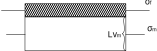
\includegraphics[width = 0.5\textwidth]{./Images/fiber_composite_parallel.eps}
	\caption{Illustration av en del av en enkelriktad fiberkomposit som belastas längsmed fiberns riktning.}
	\label{fig:fiber_composite_parallel}
\end{figure}

Kraftjämvikten ger $F = \sigma A$. Vi antar att den utskurna biten är ett rätblock, så de två delarna har tvärsnittsareor som ges av totala tvärsnittsarean och volymfraktionerna. Detta ger
\begin{align*}
	F = \sigma A = (\sigma_{\text{f}}v_{\text{f}} + \sigma_{\text{m}}v_{\text{m}})A.
\end{align*}
Därmed ges spänningen av
\begin{align*}
	\sigma = \sigma_{\text{f}}v_{\text{f}} + \sigma_{\text{m}}v_{\text{m}}.
\end{align*}
Vi antar att fibern och matrisen inte glider relativt varandra, och därmed har de samma deformation och töjning. Hookes lag ger
\begin{align*}
	\sigma_{\text{f}} = E_{\text{f}}\varepsilon, \sigma_{\text{m}} = E_{\text{m}}\varepsilon,
\end{align*}
vilket insatt i uttrycket ovan ger
\begin{align*}
	\sigma &= v_{\text{f}}E_{\text{f}}\varepsilon + v_{\text{m}}E_{\text{m}}\varepsilon \\
	       &= (v_{\text{f}}E_{\text{f}} + v_{\text{m}}E_{\text{m}})\varepsilon.
\end{align*}
För hela biten med fiberkomposit ger Hookes lag då
\begin{align*}
	E_{\text{L}} = v_{\text{f}}E_{\text{f}} + v_{\text{m}}E_{\text{m}}
\end{align*}
som elasticitetsmodulen vid längsgående spänning. Vi får även
\begin{align*}
	\sigma_{\text{f}} &= E_{\text{f}}\varepsilon \\
	                  &= \frac{E_{\text{f}}}{E_{\text{L}}}\sigma
\end{align*}
som spänning i fibrerna, och motsvarande för matrisen.

På samma sättet beskriver vi även fallet när spänningen går på tvärs av fibrernas riktning, som illustrerad i figur \ref{fig:fiber_composite_normal}.
\begin{figure}[!ht]
	\centering
	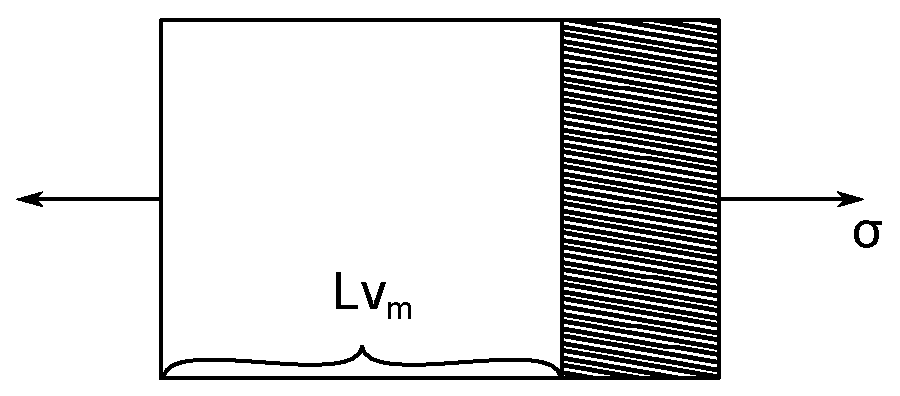
\includegraphics[width = 0.5\textwidth]{./Images/fiber_composite_normal.eps}
	\caption{Illustration av en del av en enkelriktad fiberkomposit som belastas normalt på fiberns riktning.}
	\label{fig:fiber_composite_normal}
\end{figure}

Här kan vi snitta och se att $\sigma_{\text{f}} = \sigma_{\text{m}}$. Den totala förlängningen i denna biten ges av
\begin{align*}
	\delta = \delta_{\text{f}} + \delta_{\text{m}} = L_{\text{f}}\varepsilon_{\text{f}} + L_{\text{m}}\varepsilon_{\text{m}}.
\end{align*}
Töjningen ges då av
\begin{align*}
	\varepsilon &= \frac{\delta}{L_{\text{f}} + L_{\text{m}}} \\
	            &= \varepsilon_{\text{f}}\frac{L_{\text{f}}}{L_{\text{f}} + L_{\text{m}}} + \varepsilon_{\text{m}}\frac{L_{\text{m}}}{L_{\text{f}} + L_{\text{m}}} \\
	            &= v_{\text{f}}\varepsilon_{\text{f}} + v_{\text{m}}\varepsilon_{\text{m}}.
\end{align*}
Hookes lag ger
\begin{align*}
	\varepsilon &= v_{\text{f}}\frac{\sigma}{E_{\text{f}}} + v_{\text{m}}\frac{\sigma}{E_{\text{m}}},
\end{align*}
och vi ser att
\begin{align*}
	\frac{1}{E_{T}} = \frac{v_{\text{f}}}{E_{\text{f}}} + \frac{v_{\text{m}}}{E_{\text{m}}}.
\end{align*}

\paragraph{Ideallastisk vridning}
Vi inför idealplastiska material även i vridningssammanhang. Dessa beter sig analogt till idealplastiska material under dragning, där vi ersätter töjningen med skjuvvinkeln $\gamma$, spänningen med skjuvspänningen $\tau$, töjningsgränsen med en vinkelgräns $\gamma_{\text{s}}$ och sträckgränsen med en skjuvgräns $\tau_{\text{s}}$.

\paragraph{Knäckning}
Om man t.ex. belastar en balk i dens längdriktning med en last som är större än en viss kritisk last, kommer balken snabbt böjas och nå ett nytt jämviktsläge. Detta kommer av att ursprungsläget är en instabil jämviktspunkt, så den minsta störning kommer att få den att anta ett stabilt jämviktstillstånd. Detta är ett exempel på ett instabilitetsfenomen.

\paragraph{Plasiticitetsteori i tre dimensioner}
I tre dimensioner inför vi effektivspänningen $\sigma_{\text{e}}$, som beror av spänningsmatrisen, och kräver $\sigma_{\text{e}}(S) = \sigma_{\text{s}}$ för att plasticitet skall inträda. Vi kommer undersöka detta för isotropa material.

Vi kan välja huvudspänningsriktningarna som koordinatsystem. Då kan effektivspänningen reduceras till $\sigma_{\text{e}}(S) = \sigma_{\text{e}}(\sigma_{1}, \sigma_{2}, \sigma_{3})$. Plasticitetskriteriet definierar då en yta i tre dimensioner. Av rimlighetsskäl kan ytan inte skära origo.

Vi kan kräva vissa saker av flytvillkoret, till exempel
\begin{itemize}
	\item det skall vara oberoende av eventuellt hydrostatiskt tryck, dvs. $\sigma_{\text{e}}(\sigma_{1}, \sigma_{2}, \sigma_{3}) = \sigma_{\text{e}}(\sigma_{1} - p, \sigma_{2}- p, \sigma_{3}- p) = \sigma_{\text{s}}$. Detta implicerar att ytan som definieras av flytvillkoret är en cylinderyta med riktning $(1, 1, 1)$.
	\item det uppfyller ett enaxligt flytvillkor, dvs. att om någon huvudspänning är $\sigma_{\text{s}}$ och de andra är $0$, uppfylls flytvillkoret.
	\item det är oberoende av reversering av spänningstillståndet, dvs. om alla huvudspänningar byter tecken är flytvillkoret uppfyld.
	\item det är isotropiskt, dvs. permutation av huvudspänningarna ger fortfarande att flytvillkoret är uppfyld.
\end{itemize}
Från detta kan vi dra slutsatsen att vi endast behöver titta på en $30\degree$ sektor av ytan, då symmetrier ger resten av ytan.

\paragraph{von Mises}
von Mises lösning är att säja att denna sektorn är en cirkelbåge. Det finns en formel för denna.

\paragraph{Tresca}
Trescas lösning är att säja att denna sektorn är en rät linje. Det finns en formel för denna.

\paragraph{Jämförelse}
Om man jämför Trescas och von Mises teorir, blir det störst skillnad vid ren vridning. Trescas villkor är en mer konservativ gräns än von Mises, då den allmänt ligger närmare origo. Trescas villkor har hörn, och är därför svår numeriskt. Båda funkar ändå rätt bra när man jämför med experiment.

\paragraph{Utmattning}
Utmattning är fenomenet som uppstår när brott uppstår under spänningsgränser. Det som händer är att spänningsgränsen blir lägre i materialet av cyklisk deformation, och att den tenderer mot en utmattningsgräns.

För att beskriva cykliska belastningar, inför vi begreppen minimumspänning, maximumspänning, amplitudspänning, mittspänning och spänningsförhållande. Vi har
\begin{align*}
	\sigma_{\text{a}} &= \frac{\sigma_{\text{max}} - \sigma_{\text{min}}}{2}, \\
	\sigma_{\text{m}} &= \frac{\sigma_{\text{max}} + \sigma_{\text{min}}}{2}, \\
	R                 &= \frac{\sigma_{\text{min}}}{\sigma_{\text{max}}}.
\end{align*}

\paragraph{Dragprovning och S-N-diagram}
För att testa materialers utmattningsegenskaper, kan man utsätta ett prov för varierande spänningar. Det vanlige är rent varierande eller pulserande spänningar. För en given spänningsamplitud kan man mäta hur många cykler provet kan gå igenom innan brott, och detta kan plottas i ett S-N-diagram. I ett sånt diagram kan man också rita olika kurvor för olika brottsannolikheter.

Av detta kan man läsa av brottgränsen $\sigma_{\text{B}}$ vid låga $N$ och utmattningsgränsen $\sigma_{\text{u}}$ vig höga $N$. Om man belastar provet med en spänning som är lägre än detta, har provet oändlig livslängd. Kurvan har typiskt en omvänd sigmoid form, och gränslivslängden $N{\text{g}}$ definieras som det $N$ där kurvan igen blir platt. Om spänningen är pulserande, betacknas utmattningsgränsen som $\sigma_{\text{up}}$. Motsvarande gränser kan även införas vid böjning eller böjning med rotation.

\paragraph{Haigh-diagram}
Ett Haigh-diagram är en representation av alla kombinationer av mittspänning och amplitudspänning som ger brott. Vi kommer dock förhålla oss till förenklade Haigh-diagram. Dessa konstrueras vid att dra räta linjer mellan olika punkter.

Den första punkten är $\sigma_{\text{m}} = 0, \sigma_{\text{a}} = \sigma_{\text{u}}$, som motsvarar rent växlande belastning. Den andra punkten är en rent växlande spänning $\sigma_{\text{a}} = \sigma_{\text{m}} = \sigma_{\text{up}}$. Den tredje punkten fås från ett rent statiskt dragprov $\sigma_{\text{a}} = 0, \sigma_{\text{m}} = \sigma_{\text{B}}$. Linjerna mellan dessa är ett Haigh-diagram. Man kan även förfina vid att lägga till en linje mellan $\sigma_{\text{s}}$ på båda axlarna för att ta höjd för plasticering. Då blir Haigh-diagrammet den kurvan som ligger lägst i diagrammet.

För att undersöka om den givna lasten ger brott, ritar man punkten in i Haigh-diagrammet. Om punkten är under kurvan, sker inte brott.

\paragraph{Dimensionering}
I vanliga fall vill man inte göra val baserad på gränserna utan med lite marginaler. Då kan man välja efter gränserna, fast multiplicerad med en faktor
\begin{align*}
	1 - \frac{\lambda}{K_{\text{f}}K_{\text{r}}K_{\text{d}}}.
\end{align*}
De olika faktorerna här förtjäner lite förklaring.

$\lambda$ är en faktor som tillkommer på grund av materialkvalitet. I moderna material är denna endast viktig för gjutna komponenter.

$K_{\text{f}}$ beror igen av en geometrisk faktor $K_{\text{t}}$. Tack, hållf. Om det finns variationer i komponentens tvärsnitt längsmed dens längd, beräknar man nominell spänning med hjälp av den minsta tvärsnittsdatan för att uppskatta den största spänningen som förekommer. Den maximala spänningen i komponenten är dock större än detta, tydligen, och kvoten mellan den maximala och nominella spänningen är $K_{\text{t}}$. $K_{\text{f}}$ fås med hjälp av sambandet $K_{\text{f}} = 1 + q(K_{\text{t}} - 1)$, där $q$ är en materialberoende storhet.

$K_{\text{r}}$ beskriver ytfinheten, som visar sig påverka hållfastheten. Denna beror igen av medelytavvikelsen $R_{\text{a}}$.

$K_{\text{d}}$ beror av provets storlek. Storleken spelar in på ett sätt som inte är helt klart.

När man nu har konstruerat sitt förbättrade Haigh-diagram, kan man bestämma säkerhetsfaktorer med hjälp av avstånd i Haigh-diagrammet. Hur detta görs beror på vilken sorts last man har, och beskrivs (förhoppningsvis) i formelbladet.